This chapter presents the introduction to the software metrics as the important tool for evaluation of quality and productivity of the software development product. Also the classification of the software metrics, description the different measurements of software metrics in general and the most popular software metrics tools are included in this chapter.


\section{Definition of Software Metrics}

Software metrics are the attributes of the software systems that deals with the measurements of the software product and process by which it is developed ~\cite{metrix}.
 
A software metric is a measure of characteristics of software which are countable or quantifiable. The importance of software metrics is valuable for many reasons, including planning work items, measuring software performance, measuring productivity, and many other uses.

Software developers must recognize the principles of software metrics that involve cost,schedule find quality goals, quantitative goals, comparison of plans with actual performance throughout development, monitoring data trends for indication of likely problems, metrics presentation, and investigation of data values.

There are some metrics within the process of software development, that are all related to each other. Metrics can be related to the four functions of management:

\begin{itemize}
	\item Controlling.
	\item Planning.
	\item Improving.
	\item Organising.
\end{itemize}

The aim of analyzing and tracking software metrics is to find out the quality of the particular product or process, enhance its quality and forecast the quality once the software development project is done. On a more detailed level, software development managers try to:

\begin{itemize}
	\item Manage workloads.
	\item Increase return on investment (ROI).
	\item Reduce overtime.
	\item Identify areas of improvement.
	\item Reduce costs.
\end{itemize}

These goals can be polished by providing information and clarity overall the organization about complex software development projects. Metrics are an essential value of quality assurance, performance, management, debugging, and estimating costs, and they are valuable for both development team leaders and developers:

\begin{itemize}
	\item Teams of software developers can use software metrics to interact between the status of
	software development projects, pinpoint and address issues, and observe, improve on,
	and manage their workflow better.
	\item Managers of software can use software metrics to track, identify, communicate and prioritize any
	issues to foster better team productivity. This permits effective management and allows
	prioritization and assessment of problems within software development projects. The
	sooner managers can find software problems, the easier and less-expensive the process of troubleshooting.
\end{itemize}

Software metrics provide an assessment of the impact of decisions made through the process of development of software projects. This helps managers prioritize and assess performance goals and objectives.

\section{Classification of software metrics}

Software metrics are broadly classified as product metrics and process metrics as shown in Figure \ref{fig:classification} ~\cite{metrics2}.
\begin{figure}[ht]
	\centering
	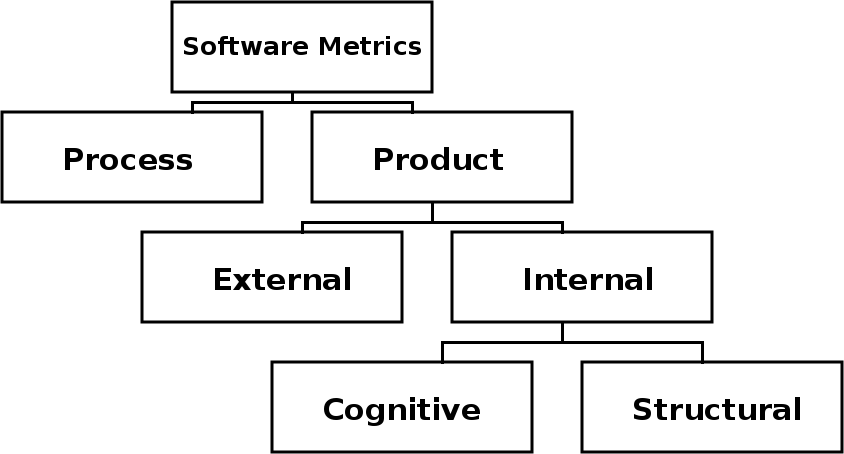
\includegraphics[height=55mm]{figures/classification.png}
	\caption{Classification of software metrics.}
	\label{fig:classification}
\end{figure}

Process metrics are numerical values that depict a software process such as the amount of time require to debug a module~\cite{metrics2}. They are measures of the software development process, such as: overall development time and type of methodology used. Process metrics are collected across all projects and over long periods of time. Their intent is to provide indicators that lead to longterm software process improvement.

Product metrics can be used to analyze and check the software project. These type of metrics calculates the complexity of the software design size of the final program number of pages of documentation produced. They allow a software project manager to do the following:

\begin{itemize}
	\item[--] decrease the development time by making the necessary modifications to avoid delays and potential problems and risks.
	\item[--] project quality assessment and change the technical approach to get better quality.
\end{itemize}

Product metrics are measures of the software product of any stage of its development,from requirements to installed system ~\cite{metrics2}. Product metrics may measure: the complexity of the software design, the size of the final program, the number of pages of documentation produced.
Product metrics can be internal or external. External attributes of an entity can be measured only with respect to how the entity relates with the environment and therefore can be measured only indirectly. For example, reliability, an external attribute of a program, does not depend only on the program itself but also on the compiler, machine and user. Productivity, an external attribute of a person, clearly depends on many factors such as the kind of process and the quality of the software delivered. Internal product metrics can be measured only based on the entity and therefore the measures are direct. For example, size is an internal attribute of any software document.

Internal product metrics are subdivided in two categories: cognitive
complexity metrics and structural complexity metrics. Cognitive complexity metrics measure the effort required by developers to understand a system. They aim at discovering the cause of the complexity, which requires understanding human mental processes and details of the software system under development. Structural complexity metrics use the interactions within and among modules to measure a system’s complexity. One of the oldest and most commonly used structural complexity metrics is the number of source lines of code.

Another classification of software metrics is as follows:

\begin{enumerate}
	\item Objective metrics.
	\item Subjective metrics
\end{enumerate}

Objective metrics always results in identical values for a given metric as measured by two or more qualified observers. Whereas subjective metrics are those that even qualified observers may measure different values for a given metric since their subjective judgment is involved in arriving at the measured value.
%%____________________________________________________________________________

\section{Types Of Software Metrics}

It is now apparent that software metrics are important in software engineering. Symons stated that "a reliable and credible method for measuring the software development cycle is needed that has a reasonable theoretica1 basis and that produces results that practitioners can trust" ~\cite{symons}. Hence, software metrics were used to measure a wide range of software developing activities.

\subsection{Size-Oriented metrics}

Size-oriented metrics are used to analyze the quality of software.

\textbf{Lines of Code (LOC)}

Lines Of Code (also possible SLOC - Source Lines of Code) is a metric generally used to measure a software program or codebase according to its size. It represents how many lines of source
code exist in the application, class, methord or namespace. LoC can be used for: checking the size of code units and estimating the size of project. LOC is the simplest one but very popular.
There are two major types of SLOC measures: 

\begin{description}
	\item[Physical SLOC (LOC)] Physical SLOC is a number of lines in the source code of the program including comment.
	\item[Logical SLOC (LLOC)] Logical LOC tries to calculate the number of "statements", but their specific definitions are tied to specific computer languages.
\end{description}

Physical SLOC measures are sensitive to logically irrelevant formatting and style conventions, while logical LOC is less sensitive to formatting and style conventions. Unfortunately, SLOC measures are often stated without giving their definition, and logical LOC can often be significantly different from physical SLOC.

\subsection{Object-oriented metrics}

Chidamber and Kemerer have specified several metrics for object-oriented designs ~\cite{ck}. All of these metrics are referred not to the whole system, but the separate class.

\textbf{Number Of Methods (NOM)}

The Number Of Methods metric is used to measure the average count of all class operations per class. A class must have some, but not an excessive number of operations. This information is useful when identifying a lack of primitiveness in class operations (inhibiting re-use), and in classes which are little more than data types.

\textbf{Number Of Children (NOC)}

NOC metric measures the number of subclasses which belong to a class. This metric calculates the class hierarchy.

NOC metric is closely relevant with DIT metric, which is more better because it supports for reusing methods through inheritance. The first metric calculates the number of child classes, DIT measures the depth of the class.
Inheritance levels can be used to gain the depth and reduce the breadth.

A high number of NOC means the following: 
\begin{itemize}
	\item Wrong abstraction of the parent class. 
	\item The reuse of the base class is high. The form of reuse is inheritance.
	\item Wrong using of subclasses. In this case, it is needed to introduce a new level of inheritance with newly grouped related classes.
	\item Base class needed to be more tested.
\end{itemize}

Classes high hierarchy have more subclasses then classes with low hierarchy. The number of children gives an idea of the potential influence a class has on the design ~\cite{ck}.

\textbf{Weighted Methods per Class (WMC)}

This metric calculates a sum of complexities all defined methods in a class. WMC shows the complexity of whole class. This measure helps to indicate the development and maintenance effort for the class. Classes with a large number of WMC can often be refactored into several classes.

A class with a high value of WMC and a high number of NOC indicates complexity at the top of the class hierarchy. A sign of poor design is the potential impact of the base class on a large number of subclasses.

\textbf{Coupling Between Object classes (CBO)}

CBO classes metric demonstrates the number of classes coupled to a given class. This coupling can happen through:
\begin{itemize}
	\item Properties or parameters. 
	\item Method call. 
	\item Method arguments or return types.
	\item Class extends.
	\item Variables in methods
\end{itemize}

Coupling among classes is crucial for a system to do useful work, but redundant coupling makes the system more complicated to maintain and reuse. At the project or package level, this metric displays the average number of classes used per class. A measure of coupling is useful to determine how complex the testing of various parts of a design are likely to be ~\cite{ck}.

\textbf{Depth of Inheritance Tree (DIT)}

Depth of Inheritance Tree (DIT) measures the maximum length of a path from the current class to the root class in the inheritance structure of a system. DIT calculates how many super-classes can affect a class. DIT is applicable only to object-oriented systems.

If a class is on the deep level in the hierarchy, the more methods and variables it tends to inherit, what makes it more complex. Deep trees indicate big complexity of the design. Inheritance is a key for complexity managing, really, not for its increasing. As a positive factor, deep trees promote reuse because of method inheritance. Deeper trees constitute greater design complexity, since more methods and classes are involved ~\cite{ck}.

C\&K suggested the following consequences based on the depth of inheritance:
\begin{itemize}
	\item Deeper trees establish large design complexity, since more classes and methods are involved
	\item If a class is on the deep level in the hierarchy, the more methods and variables it tends to inherit, what makes it more complex to foresee its behavior
	\item If a particular class is on the deep level in the hierarchy, there is a great chance of the possible reuse of inherited methods 
\end{itemize}

\textbf{Response For a Class (RFC)} 

The Response for Class (RFC) metric measures the total number of methods that can probably be executed as a response to a message received by some object of a class. This number calculates as the sum of the methods of the class, and all distinct methods are called directly within the class methods. Additionally, it counts inherited methods, but not overridden methods, because only one method of a particular signature will always be accessible for an object of a given class.

A large RFC is an indicator of more faults. Classes that have a high RFC are more complex and more difficult to understand. Testing and debugging for these classes is also complicated. A worst-case value for possible responses will assist in the appropriate allocation of testing time. If a large number of methods can be invoked on response to a message, the testing and debugging of the class becomes more complicated since it requires a greater level of understanding required on the pan of the tester ~\cite{ck}.
%%___________________________________________________
\subsection{Complexity metrics}

Complexity is an important aspect for software quality assessment and must be appropriately addressed in service-oriented architecture ~\cite{complexity}. One of the key aims of complexity  metrics is to predict modules that are fault-prone post-release ~\cite{complexity2}. These metrics are one of the most difficult software metrics for understanding.

\textbf{McCabe's Cyclomatic Complexity (MVG)}

To determine the complexity of a software, McCabe suggests a "mathematical technique that will provide a quantitative basis for modularisation and allow us to identifY software modules that will be difficult to test or maintain" ~\cite{shepperd}. McCabe's cyclomatic complexity ~\cite{mc} is a software quality metric that shows the complexity of a software program. Complexity is inferred by summarizing the number of linearly independent paths through the program. The higher the number the more complex the code.

A pragmatic approximation to this can be found by counting language keywords and operators which introduce extra decision outcomes.
%%_______________________________
\subsection{Structural Metrics}

\textbf{Fan-In and Fan-Out metrics (FIN and FOUT)}

It is a structural metrics which measures inter-module complexities. 
\begin{description}
	\item[Fan-out] Is the number of modules that are called by a given module.
	\item[Fan-in] Is the number of modules that call a given module.
\end{description}

Fan-out and fan-in metrics reflect structure dependency ~\cite{fanin}.
These structural metrics were first defined by Henry.
These metrics can be applied both at the module level and function level. These metrics just put a number on how complex is interlinking of different modules or functions. Unlike Cyclomatic complexity, you cannot put a number and say it cannot go beyond this number. This is used just to size up how difficult it will be to replace a function or module in your application and how changes to a function or module can impact other functions or modules. Sometimes you can put the restriction on the number of Fan-Out.

%%______________________________________________________

\subsection{Cohesion metrics}
Cohesion is an important software quality attribute and high cohesion is one of the characteristics of well-structured software design ~\cite{cohesion}.
Cohesion metrics analyze the connection between the methods of a class.
Module cohesion indicates relatedness in the functionality of a software module ~\cite{cohesion2}.

\textbf{Lack of Cohesion in Methods (LCOM)}

LCOM calculates the number of cohesiveness present, how well a system was designed and how complex a class is. LCOM is a count of the number of method pairs whose similarity is zero, minus the count of method pairs whose similarity is not zero. LCOM is probably the most controversial and argued over of the C\&K metrics.

C\&K's rationale for the LCOM method was as follows:
\begin{itemize}
	\item Lack of cohesion implies classes should probably be split into two or more subclasses.
	\item The cohesiveness of methods within a class is desirable since it promotes encapsulation.
	\item Low cohesion increases complexity, thereby increasing the likelihood of errors during the development process.
	\item Any measure of disparateness of methods helps identify flaws in the design of classes. 
\end{itemize}

Although there is a fair amount of debate about how to calculate LCOM and it features in a lot of metrics sets an increasing number of researchers to suggest that it is not a particularly useful metric. Perhaps this is also reflected in there being a fair amount of debate about how to calculate LCOM but very little on how to interpret it and how it fits in with other metrics. 

\textbf{Tight and Loose Class Cohesion (TCC and LCC)}

TCC (Tight Class Cohesion) and LCC (Loose Class Cohesion) metrics measure the relative number of directly-connected pairs of methods and the relative number of directly- or indirectly- connected pairs of methods.
The Tight Class Cohesion metric measures the cohesion between the public methods of a class. That is the relative number of directly connected public methods in the class. Classes having a low cohesion indicate errors in the design.

TCC considers two methods to be connected if they share the use of at least one attribute. A method uses an attribute if the attribute appears in the method’s body or the method invokes directly or indirectly another method that has the attribute in its body. The higher TCC and LCC, the more cohesive and thus better the class.

In this Section, we focused our attention on all possible software metrics. In the next Chapter, we will define metrics which are used to describe various aspects of Erlang projects. 
%%______________________________________________________________________

\section{Software Metric Tools}
There are a lot of software metrics have been developed and numerous tools exist to gather the metrics from program representations. This large number of tools allows a user to choose the tool best suited for user requirements, for example, its handling, tool support, cost etc. This is accepted that the metrics computed by the metric tools are the same for all the metric tools. One can think of a software metric tool as a program which implements a set of software metrics definitions. It allows accessing a software system according to the metrics by extracting the required entities from the software and providing the corresponding metric values. There are
some criteria for selecting the proper metric tools as the availability of the software tools can make confusion. One such criterion is that the tools must have to calculate any form of software metrics. Majority metric tools are available for Java programs. Many tools are just code counting
tool, they basically count the variants of the lines of code (LOC) metric. The specific criteria areas follow language: Java (source or bytecode), metrics: well-known object-oriented metrics on class level, license: freely available.

\subsection{CCCC}

CCCC is a small command-line tool which generates metrics from C or C++ project's source code ~\cite{cccc}. The tool outputs a simple HTML website with information about all your sources. It generates reports on different metrics, for example, lines of code (LOC) and metrics suggested by Chidamber\&Kemererand Henry\&Kafura. CCCC is distributed as a freeware and is released in the form of source code. Users have to compile the program on their own and to modify the source code to reflect their interests and preferences.

CCCC can process every file which was provided via the command line. It is possible to use standard wildcard process. For every file, CCCC will check the filename's extension, and if the extension is recognized as one from supported languages, the particular parser will parse this file. As every file is parsed, certain constructs recognition will cause records to be inserted into an internal database. After all files have been processed, the software will generate the report in HTML format. This report is depended on on the contents of the internal database. By default settings the main HTML report is produced to the file cccc.htm in a subfolder called .cccc of the current working folder. It includes detailed reports on every module (for example, C++ or Java class) detected by the analysis run.

As an addition to HTML reports and summary, the run of the program will generate the corresponding summary and reports in XML format. Also, the file called cccc.db will be created. This file will represent a dump of the internal database of the software in a special format with '@' symbol as a delimiter. It is chosen because this symbol is one of the few which can not appear in C/C++ source code.

The report consists of a number of tables which identify the modules in the submitted files and covering:
\begin{enumerate}
	\item Measures the number and the relationships type.
	\item Measures the procedural volume and complexity and functions of every module. 
	\item A summary report over the whole codebase processed of the measures described above.
	\item Identification of any parts of the source code submitted which the program can not parse.
\end{enumerate}

This tool can measure the following metrics:
\begin{itemize}
	\item Fan-In Fan-Out (FIN and FOUT).
	\item Lines of Code (LOC). 
	\item Number Of Children (NOC).
	\item Weighted Methods per Class (WMC).
	\item McCabe's Cyclomatic Complexity (MVG).
	\item Number Of Methods (NOM).
\end{itemize}

\subsection{Chidamber\&Kemerer}

The program counts Chidamber and Kemerer object-oriented metrics by introspection the bytecode of compiled Java files ~\cite{ck1}. It is an open source command line tool. The program counts the following six metrics for each class, and displays them on its standard output, following the class's name.

This tool can measure the following metrics:

\begin{itemize}
	\item Depth of Inheritance Tree (DIT).
	\item Weighted Methods per Class (WMC).
	\item Numbe r Of Children (NOC).
	\item Coupling Between Object classes (CBO).
	\item Lack of Cohesion in Methods (LCOM).
	\item Response For a Class (RFC).
\end{itemize}

\subsection{Analyst4j}
Analyst4j is built on the Eclipse platform and can be downloaded as a standalone Rich Client Application or also as an Eclipse
IDE plugin ~\cite{analyst4j}. Its features are search, metrics analyzing, quality analyzing, report generating for Java programming.
Analyst4j software is most popular to find out the quality-related metrics. This tool is based on Chidamber\&Kemerer metrics.

This tool can measure the following metrics:
\begin{itemize}
	\item Weighted Methods per Class (WMC).
	\item Lines of Code (LOC). 
	\item Coupling Between Object classes (CBO).
	\item Depth of Inheritance Tree (DIT).
	\item Response For a Class (RFC).
	\item Number Of Children (NOC).
	\item Lack of Cohesion in Methods (LCOM).
	\item Number Of Methods (NOM).
\end{itemize}

\subsection{OOMeter}

OOMeter is a software metric tool for measuring the quality attributes of Java and C\# source code and UML models, stored in XMI format ~\cite{meter}. OOMeter has a rich collection of object-oriented software metrics. This is the Eclipse plugin. It provides a querying language for object-oriented code similar to SQL which allows to search for measure code metrics, bugs etc.

OOMeter provides an interface for users to define custom metrics through Java classes that implement a certain interface. It supports export of metric results to a number of formats, including XML, HTML, delimited text, Microsoft Excel, etc ~\cite{meter2}.

This tool can measure the following metrics:

\begin{itemize}
	\item Weighted Methods per Class (WMC).
	\item Lines of Code (LOC). 
	\item Coupling Between Object classes (CBO).
	\item Depth of Inheritance Tree (DIT).
	\item Response For a Class (RFC).
	\item Numbe r Of Children (NOC).
	\item Tight Class Cohesion (TCC).
	\item Lack of Cohesion in Methods (LCOM).
\end{itemize}



\subsection{Eclipse Metrics plugin 1.3.6}

This is an open source dependency analyzer and metrics calculation plugin for Eclipse IDE ~\cite{ecl}. The plugin is also provided integrated as an EasyEclipse package. The plugin computes the various metrics and displays it in the integrated view.


This tool can measure the following metrics:

\begin{itemize}
	\item Weighted Methods per Class (WMC).
	\item Lines of Code (LOC). 
	\item Numbe r Of Children (NOC).
	\item Depth of Inheritance Tree (DIT).
    \item Number Of Methods (NOM).
\end{itemize}

\subsection{Eclipse Metrics plugin 3.4}
The eclipse plugin 3.4 developed by Lance Walton is also integrated with Eclipse and is available for all Java projects developed using the IDE ~\cite{ecl1}. It is an open source tool. It counts various metrics in the moment of build cycles and shows warnings via the problem view of metrics range violations.

This tool can measure the following metrics:
\begin{itemize}
	\item Weighted Methods per Class (WMC).
	\item Lines of Code (LOC). 
	\item Lack of Cohesion in Methods (LCOM).
	\item Depth of Inheritance Tree (DIT).
\end{itemize}

\subsection{Semmle}

Semmle is the platform for analyzing that produces a detailed report of the code base for one or more software projects ~\cite{semmle}. For every project that it analyzes, it calculates artifacts against rules that check for good practice. Analysis can be scheduled to run on a regular basis. The copy of the source code is checked out from the repository for analysis as part of this process. The code, and related artifacts is checked against rules, defined using queries, to identify any alerts. Finally, metrics are calculated and data can be imported from third-party systems used by your company. A database is created, containing detailed information about the artifacts and every alert.

This tool can measure the following metrics:
\begin{itemize}
	\item Lack of Cohesion in Methods (LCOM).
	\item Depth of Inheritance Tree (DIT).
	\item Number Of Methods (NOM).
	\item Numbe r Of Children (NOC).
	\item Response For a Class (RFC).
\end{itemize}

\section{Measuring functional languages}

In the previous section has been described software metrics for object-oriented languages. However, software metrics developed for imperative and object-oriented languages can also be used for measuring in functional programming languages like Erlang and Haskell. 

Some  of  the  measurement  techniques  from  imperative  and object-oriented  languages  may  transfer  quite  cleanly  to  functional  languages,  for  instance  the  path  count  metric  which  counts  the  number  of  execution  paths through  a  piece  of  program  code,  but  some  of  the  more  advanced features  of  functional  programming  languages  may contribute  to  the  complexity  of  a  program  in  ways  that  are  not  considered  by  traditional  imperative  or  object  oriented 
metrics ~\cite{fp}. 

We can use the same metrics because several constructs as a class, a module, and a library are similar. All of this structures can be consider like collections of functions. If the chosen metric does not take the distinctive properties of these constructs into account (variables, method overrides, dynamic binding, visibility etc.), then it can be applied to these apparently diverse constructs ~\cite{metrics3}.

The dissimilarity between functional and imperative languages are in the difference in the level of nesting of blocks and control structures, in several ways of connecting certain functions (for example, data flow and call graph), inheritance instead of cohesion and simple cardinality metrics(lines of code, char of code).

Another difference functional programming languages from imperative languages is there are some constructs and properties that can be used only in functional programming languages as list comprehensions, pattern matching, referential transparency of pure functions, currying, laziness of expression evaluation.

While these features raise the expressive power of functional languages,
most of the existing complexity metrics require some changes before they become applicable to functional languages ~\cite{metrics3}.

There are general metrics are acceptable for functional languages:
\begin{itemize}
	\item \textbf{Branches of recursion}. This metric allows measuring how many times did the function call itself
	\item \textbf{Fun expressions and message passing constructs}.
	\item \textbf{Return points of a function}.
	\item There is possible to calculate metrics on a single clause of a function.
	\item There is possible to calculate metrics on a single clause of a function.
	\item \textbf{Otp used}. This metric allows measure OTP behaviors.
\end{itemize}

In the next chapter will be described all developed metrics for Erlang in details.



